\chapter{HASIL DAN PEMBAHASAN}

\section{Hasil Exploratory Data Analysis}
\label{sec:hasil-eda}

\noindent Tahap Exploratory Data Analysis (EDA) dilakukan untuk memahami karakteristik dataset citra jaringan ginjal secara mendalam. Tujuan utama EDA adalah untuk mengidentifikasi distribusi kelas, mengidentifikasi ketidakseimbangan kelas, dan menemukan pola-pola yang mungkin mempengaruhi kinerja model. Informasi yang diperoleh dari EDA akan digunakan menentukan teknik preprocessing yang tepat pada data sehingga model yang dilatih dapat memberikan hasil yang optimal.

\subsection{Distribusi Citra dalam Dataset}
\noindent Terdapat 1633 citra jaringan ginjal manusia yang telah dilabeli dalam penelitian ini. Citra-citra tersebut terbagi menjadi dua dataset utama. Dataset pertama terdiri dari 2 sumber Whole Slide Imaging (WSI) yang berbeda, sedangkan dataset kedua berasal dari 4 sumber WSI yang berbeda. Diagram di bawah menunjukkan distribusi jumlah citra pada setiap dataset dan kombinasi dataset-sumber WSI.

\begin{figure}[H]
	\centering
	\begin{subfigure}[b]{0.4\textwidth}
		\centering
		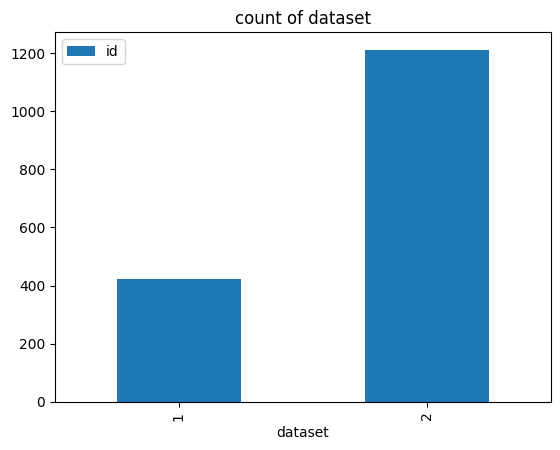
\includegraphics[width=\textwidth]{gambar/bab4/dataset.png}
		\caption{Sebaran citra dalam dataset}
		\label{fig:d_dataset}
	\end{subfigure}
	\hspace{0.05\textwidth}
	\begin{subfigure}[b]{0.4\textwidth}
		\centering
		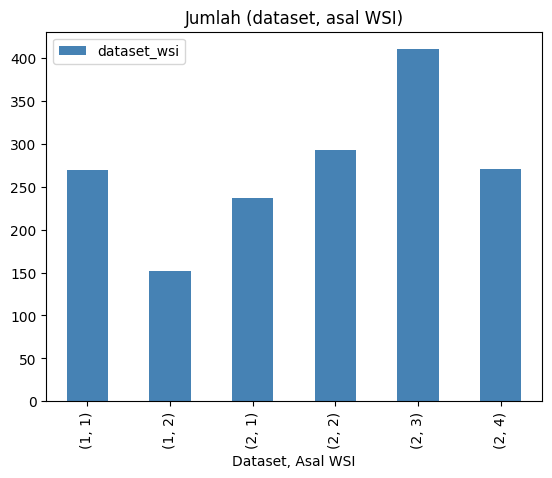
\includegraphics[width=\textwidth]{gambar/bab4/dataset_wsi.png}
		\caption{Sebaran citra dalam sumber WSI}
		\label{fig:d_WSI}
	\end{subfigure}	
	\caption{Sebaran citra pada tiap dataset dan sumber WSI}
	\label{fig:diagram_sebaran}
\end{figure}

\noindent Seperti yang terlihat pada Gambar \ref{fig:d_dataset}, dataset pertama memiliki jumlah citra yang lebih banyak dibandingkan dataset kedua. Sebaran citra pada masing-masing sumber WSI dalam kedua dataset cukup merata setelah ditampilkan berdasarkan asal sumbernya. Selanjutnya, observasi dilakukan untuk menganalisis karakteristik pembuluh darah dari masing-masing sumber WSI pada dataset 1 dan dataset 2 yang bisa dilihat pada lampiran.


\noindent Hasil observasi menunjukkan adanya perbedaan karakteristik pembuluh darah pada dataset 1 yang berasal dari source 1 dan source 2. Pembuluh darah pada source 1 cenderung berjumlah sedikit namun memiliki ukuran yang besar, sedangkan pada source 2, pembuluh darah lebih banyak tetapi berukuran kecil. Sebaliknya, pada dataset 2 yang berasal dari source 1 hingga source 4, tidak ditemukan karakteristik tertentu yang konsisten, karena setiap sampel menunjukkan variasi pembuluh darah yang sangat beragam.

\subsection{Ekplorasi Ukuran Piksel dan Kuantitas Pembuluh Darah}

\noindent Selanjutnya, distribusi ukuran rata-rata (\textit{mean size}) piksel pembuluh darah (dalam ribuan piksel) dan jumlah pembuluh darah (\textit{n$\_$bloodVessel}) untuk setiap sumber dataset dapat dilihat pada Gambar  Scatter plot ini menunjukkan pola distribusi yang berbeda di antara sumber-sumber dataset.

\begin{figure}[H]
	\centering
	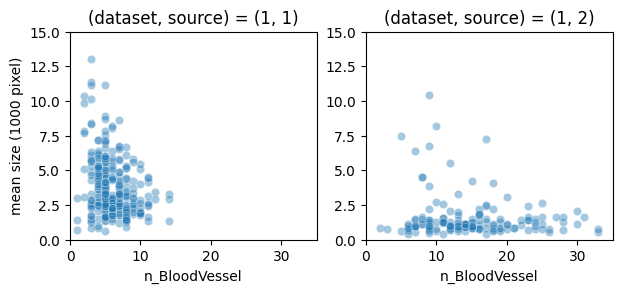
\includegraphics[width=\textwidth]{gambar/bab4/sct_1.png}
	\caption{Sebaran ukuran dan kuantitas pembuluh darah dataset 1}
	\label{fig:sct_1}
\end{figure}

\noindent Pada sumber 1 dan 2, terlihat bahwa jumlah pembuluh darah umumnya berkisar antara 0 hingga 30, dengan ukuran rata-rata piksel pembuluh darah yang cenderung kecil (<5 ribu piksel). Pada sumber 1 terlihat bahwa jumlah pembuluh darah lebih sedikit namun rata-rata piksel pembuluh darah lebih bersar dari sumber 2.

\begin{figure}[h]
	\centering
	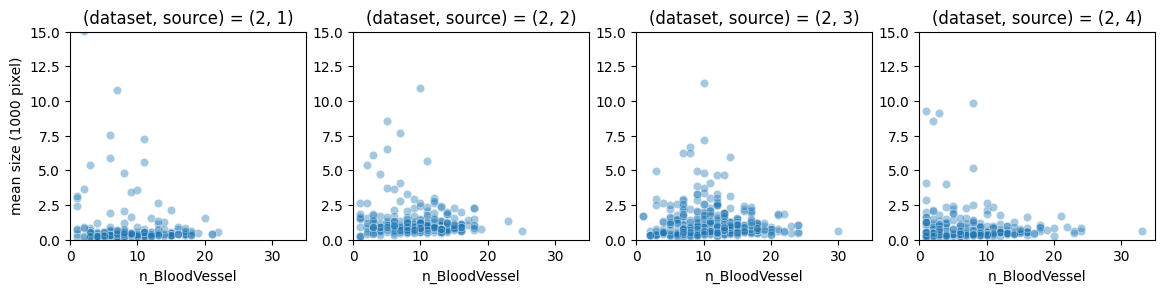
\includegraphics[width=\textwidth]{gambar/bab4/sct_2.png}
	\caption{Sebaran ukuran dan kuantitas pembuluh darah dataset 2}
	\label{fig:sct_2}
\end{figure}

\noindent Distribusi pada dataset 2 lebih beragam dibandingkan dataset 1. Ukuran rata-rata pembuluh darah pada sumber 1 hingga 4 umumnya lebih kecil daripada dataset 1, dengan sebagian besar pembuluh darah berukuran kurang dari 5 ribu piksel.


\subsection{Distribusi label pada dataset}
\noindent Berdasarkan analisis terhadap keseluruhan label dalam dataset, hanya sekitar 5$\%$ label yang merepresentasikan object (pembuluh darah), sedangkan sisanya merupakan latar belakang. Distribusi rata-rata rasio label positif (pembuluh darah) terhadap total label untuk setiap sumber (source WSI) dirangkum pada Tabel berikut:


\begin{table}[H]
	\centering
	\caption{Distribusi rata-rata rasio label positif pada setiap source WSI.}
	\label{tab:distribusi_label}
	\begin{tabular}{cll}
		\hline
		\multicolumn{1}{l}{Dataset} & Source WSI & Positive Ratio \\ \hline
		\multirow{2}{*}{1}          & 1          & 0.083776      \\
		& 2          & 0.084165       \\ \hline
		\multirow{4}{*}{2}          & 1          & 0.024374       \\
		& 2          & 0.048241       \\
		& 3          & 0.047921       \\
		& 4          & 0.023660       \\ \hline
	\end{tabular}
\end{table}

\noindent Dari tabel \ref{tab:distribusi_label} terlihat bahwa distribusi rasio label positif bervariasi antara dataset dan sumber WSI. Dataset 1 memiliki rasio rata-rata label positif yang lebih tinggi (sekitar 8$\%$) dibandingkan dengan dataset 2, di mana rata-rata rasio label positif berkisar antara 2$\%$ hingga 5$\%$. Hal ini menunjukkan adanya ketidakseimbangan kelas yang signifikan dalam dataset, dengan mayoritas piksel pada citra merupakan latar belakang.


\section{Hasil Pelatihan dan Evaluasi}
\noindent Setelah memahami karakteristik dataset melalui Ekplolatory Data Analisys (EDA), model dilatih menggunakan konfigurasi praprosessing dan hyperparameter yang telah ditentukan di Bab \ref{sec:metode-penelitian} Metode Penelitian. Bagian ini akan menyajikan hasil training dan evaluasi model Attention U-Net serta pembandingnya, U-Net, untuk tugas segmentasi mikrovaskular ginjal. Pada tabel \ref{tab:training-results} disajikan seluruh metrik hasil pelatihan.

\begin{landscape}
\begin{table}[]
	\caption{Hasil pelatihan model Attention U-Net dan U-Net dengan berbagai konfigurasi hyperparameter}
	\label{tab:training-results}
	\begin{tabular}{@{}llllllllllll@{}}
		\toprule
		Model &
		Optimizer &
		Batch Size &
		Oversample &
		DSC &
		IoU &
		Recall &
		Precision &
		Train Loss &
		Val Loss &
		Learning Rate &
		Epotch \\ \midrule
		\multirow{10}{*}{Attention U-net} &
		\multirow{5}{*}{SGD} &
		4 &
		Tidak &
		0.362 &
		0.239 &
		0.335 &
		0.488 &
		0.803 &
		0.817 &
		4.0e-5 &
		33 \\
		&  & 8  & Tidak & 0.265          & 0.168          & 0.264          & 0.429          & 0.983 & 1.002  & 2.0e-4 & 49 \\
		&  & 16 & Tidak & 0.181          & 0.113          & 0.152          & 0.445          & 1.027 & 1.055  & 2.0e-4 & 49 \\ \cmidrule(l){3-12} 
		&  & 4  & Ya    & 0.506          & 0.363          & 0.461          & 0.641          & 0.626 & 0.611  & 8.0e-6 & 29 \\
		&  & 8  & Ya    & 0.478          & 0.337          & 0.442          & 0.590          & 0.659 & 0.6441 & 3.2e-7 & 42 \\ \cmidrule(l){2-12} 
		&
		\multirow{5}{*}{Adam} &
		4 &
		Tidak &
		\textbf{0.56} &
		\textbf{0.413} &
		\textbf{0.527} &
		\textbf{0.675} &
		0.53 &
		0.554 &
		1.6e-6 &
		27 \\
		&  & 8  & Tidak & 0.546          & 0.34           & 0.509          & 0.656          & 0.555 & 0.569  & 1.6e-6 & 37 \\
		&  & 16 & Tidak & 0.556          & 0.409          & 0.534          & 0.642          & 0.541 & 0.553  & 8.0e-6 & 29 \\ \cmidrule(l){3-12} 
		&  & 4  & Ya    & \textbf{0.624} & \textbf{0.481} & \textbf{0.595} & \textbf{0.714} & 0.404 & 0.443  & 8.0e-6 & 24 \\
		&  & 8  & Ya    & 0.617          & 0.473          & 0.597          & 0.692          & 0.412 & 0.455  & 8.0e-6 & 25 \\ \midrule
		\multirow{10}{*}{U-net} &
		\multirow{5}{*}{SGD} &
		4 &
		Tidak &
		0.521 &
		0.375 &
		0.48 &
		0.644 &
		0.592 &
		0.601 &
		7.9e-5 &
		25 \\
		&  & 8  & Tidak & 0.396          & 0.268          & 0.346          & 0.572          & 0.764 & 0.767  & 2.0e-4 & 49 \\
		&  & 16 & Tidak & 0.425          & 0.29           & 0.386          & 0.564          & 0.713 & 0.724  & 1.2e-7 & 39 \\ \cmidrule(l){3-12} 
		&  & 4  & Ya    & 0.521          & 0.376          & 0.492          & 0.625          & 0.602 & 0.59   & 1.6e-6 & 38 \\
		&  & 8  & Ya    & 0.510          & 0.367          & 0.475          & 0.620          & 0.598 & 0.605  & 8.0e-6 & 40 \\ \cmidrule(l){2-12} 
		&
		\multirow{5}{*}{Adam} &
		4 &
		Tidak &
		\textbf{0.545} &
		\textbf{0.398} &
		\textbf{0.51} &
		\textbf{0.66} &
		0.557 &
		0.57 &
		1.6e-6 &
		28 \\
		&  & 8  & Tidak & 0.54           & 0.396          & 0.503          & 0.655          & 0.549 & 0.567  & 8.0e-6 & 21 \\
		&  & 16 & Tidak & 0.544          & 0.397          & 0.516          & 0.651          & 0.534 & 0.572  & 1.6e-6 & 36 \\ \cmidrule(l){3-12} 
		&  & 4  & Ya    & \textbf{0.616} & \textbf{0.472} & \textbf{0.59}  & \textbf{0.700} & 0.424 & 0.451  & 3.2e-7 & 29 \\
		&  & 8  & Ya    & 0.612          & 0.467          & 0.593          & 0.687          & 0.432 & 0.456  & 1.6e-6 & 24 \\ \bottomrule
	\end{tabular}
\end{table}
\end{landscape}

\subsection{Hasil Pelatihan Tanpa Oversampling}

\noindent Subbab ini membahas konfigurasi terbaik yang diperoleh pada model Attention U-Net tanpa penggunaan teknik oversampling. Konfigurasi terbaik dipilih berdasarkan nilai train loss dan validation loss terendah, serta pola penurunan loss yang stabil selama pelatihan.

\noindent Berdasarkan hasil eksperimen, konfigurasi terbaik diperoleh dengan optimizer Adam dan batch size 4. Konfigurasi ini menghasilkan train loss sebesar 0.530 dan validation loss sebesar 0.554. Hal ini menunjukkan bahwa konfigurasi ini lebih stabil dibandingkan konfigurasi lain, sebagaimana ditunjukkan pada Gambar \ref{fig:loss_attention_terbaik}.

\begin{figure}[H]
	\centering
	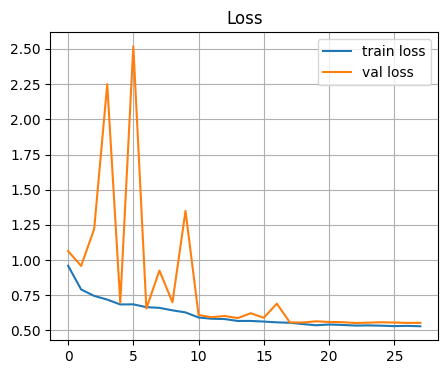
\includegraphics[scale=.8]{gambar/bab4/loss_adam_attention_u-net_4.png}
	\caption{Penurunan training loss dan validation loss pada konfigurasi Attention U-Net terbaik (optimizer Adam, batch size 4).}
	\label{fig:loss_attention_terbaik}
\end{figure}

\noindent Gambar \ref{fig:loss_attention_terbaik} menunjukkan bahwa training loss mengalami penurunan konsisten hingga mencapai konvergensi pada epoch ke-27, dengan learning rate sebesar 1.6e-6. Pola serupa juga terlihat pada validation loss, meskipun terdapat sedikit fluktuasi di epoch awal. Tidak ditemukan indikasi overfitting, karena selisih antara training loss dan validation loss tetap kecil. Penggunaan early stopping membantu menghentikan pelatihan sebelum overfitting terjadi, sehingga validasi tetap konsisten.

\noindent Sebagai perbandingan, konfigurasi dengan optimizer SGD dan batch size 4 menghasilkan train loss sebesar 0.803 dan validation loss sebesar 0.817. Nilai ini lebih tinggi dibandingkan konfigurasi terbaik, menunjukkan bahwa optimizer Adam mampu memberikan stabilitas yang lebih baik dibandingkan SGD. Stabilitas ini didukung oleh kemampuan Adam dalam mengatur gradien selama proses pelatihan.


\subsection{Evaluasi Kinerja Model dalam Segementasi}

\noindent Subbab ini mengevaluasi kinerja model Attention U-Net dan U-Net berdasarkan metrik utama, yaitu Dice Similarity Coefficient (DSC), Intersection over Union (IoU), precision, dan recall. Evaluasi dilakukan untuk berbagai konfigurasi, termasuk variasi batch size dan optimizer, dengan tujuan mengidentifikasi konfigurasi terbaik untuk setiap arsitektur. Tabel \ref{tab:training-results} menyajikan hasil lengkap dari semua eksperimen, di mana performa terbaik ditandai dengan cetak tebal untuk memudahkan interpretasi.

\noindent Berdasarkan hasil pada Tabel \ref{tab:training-results}, model Attention U-Net secara konsisten menunjukkan performa yang lebih baik dibandingkan U-Net pada semua metrik utama. Konfigurasi terbaik untuk Attention U-Net menggunakan optimizer Adam dan batch size 4 menghasilkan DSC sebesar 0.560 dan IoU sebesar 0.413. Sebagai perbandingan, konfigurasi terbaik untuk U-Net (optimizer Adam, batch size 4) hanya mencapai DSC sebesar 0.545 dan IoU sebesar 0.398. Perbedaan ini mengindikasikan bahwa penambahan mekanisme attention gate pada U-Net berkontribusi signifikan dalam meningkatkan kemampuan segmentasi.

\noindent Selain itu perbedaan kinerja juga terlihat pada precission dan recal. Attention U-net precission lebih tinggi dibandingkan dengan U-net (0.675 vs 0.660 pada U-net), menunjukkan bahwa model ini lebih baik dalam menghindari false positive. Kemudian, recall pada Attention U-net juga lebih sedikit lebih tinggi dibandingkan dengan U-net (0.527 vs 0.510 pada U-net) menunjukkan kemampuan Attention U-net yang lebih baik dalam mendeteksi pembuluh darah kecil.

\noindent Hasil ini mendukung hipotesis bahwa Attention U-Net lebih unggul dalam tugas segmentasi mikrovaskular ginjal dibandingkan U-Net. Mekanisme attention gate membantu model memfokuskan pada area yang relevan, sehingga meningkatkan akurasi segmentasi secara keseluruhan. Dengan DSC mencapai 0.560 pada konfigurasi terbaik, model Attention U-Net menunjukkan kemampuan yang dapat diandalkan untuk tugas segmentasi mikrovaskular pada Whole Slide Images (WSI) jaringan ginjal manusia. Selain itu, hasil ini juga menyoroti pengaruh signifikan penambahan modul attention gate dalam meningkatkan kinerja U-Net, sejalan dengan tujuan penelitian ini.


\subsection{Dampak Oversampling pada Ketidakseimbangan Kelas}

\noindent Berdasarkan hasil pada subbab \ref{sec:hasil-eda} Hasil Exploratory Data Analysis ditemukan bahwa proporsi piksel latar belakang jauh lebih besar dibandingkan piksel pembuluh darah. Ketidakseimbangan ini dapat menyebabkan model bias terhadap kelas mayoritas, sehingga menurunkan kemampuan model untuk mendeteksi struktur pembuluh darah yang kecil. Untuk mengatasi masalah ini, dilakukan teknik oversampling pada dataset pelatihan, yang bertujuan meningkatkan jumlah sampel dari kelas minoritas melalui augmentasi data.


\noindent Tabel \ref{tab:training-results} menyajikan perbandingan kinerja model Attention U-Net pada eksperimen dengan dan tanpa oversampling. Hasil menunjukkan bahwa oversampling memiliki dampak yang signifikan terhadap beberapa metrik utama.

\noindent Berdasarkan hasil pada Tabel \ref{tab:training-results}, penggunaan oversampling pada Attentioin U-net menghasilkan peningkatan yang signifikan pada DSC (dari 0.560 menjadi 0.624) dan IoU (dari 0.413 menjadi 0.481). Hal ini menunjukkan bahwa oversampling membantu model untuk lebih akurat dalam memetakan struktur pembuluh darah, meskipun jumlah piksel pembuluh darah jauh lebih sedikit dibandingkan latar belakang. Peningkatan recall (dari 0.527 menjadi 0.595) juga mengindikasikan bahwa oversampling meningkatkan kemampuan model dalam mendeteksi pembuluh darah kecil.

\noindent Kemudian, oversampling juga sedikit meningkatkan nilai precision (dari 0.674 menjadi 0.714), meskipun peningkatan ini relatif lebih kecil dibandingkan recall. Hal ini menunjukkan bahwa oversampling dapat memperbaiki ketidakseimbangan kelas tanpa meningkatkan jumlah false positive secara signifikan.


\section{Hasil Segmentasi Mikrovaskular}

\noindent Berdasarkan evaluasi kuantitatif pada subbab sebelumnya, model Attention U-Net menunjukkan performa yang lebih unggul dibandingkan U-Net dalam tugas segmentasi mikrovaskular ginjal, dengan peningkatan pada metrik utama seperti Dice Similarity Coefficient (DSC), Intersection over Union (IoU), precision, dan recall. Nilai DSC sebesar 0.624 menunjukkan kemampuan model yang moderat dalam mendeteksi area pembuluh darah yang hampir sesuai dengan ground truth. Sementara itu, nilai IoU sebesar 0.413 mengindikasikan adanya tantangan dalam segmentasi, terutama karena tingginya jumlah false negative pada pembuluh darah besar, sebagaimana terlihat dalam visualisasi hasil berikut.


\begin{figure}[H]
	\centering
	\begin{subfigure}[b]{0.24\textwidth}
		\centering
		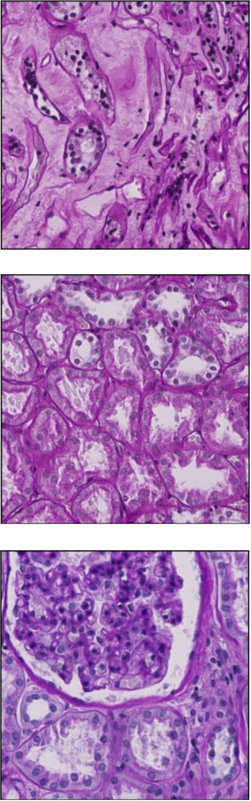
\includegraphics[width=\textwidth]{gambar/bab4/image_hasil.png}
		\caption{Citra test}
		\label{fig:image_hasil}
	\end{subfigure}
	\hfill
	\begin{subfigure}[b]{0.24\textwidth}
		\centering
		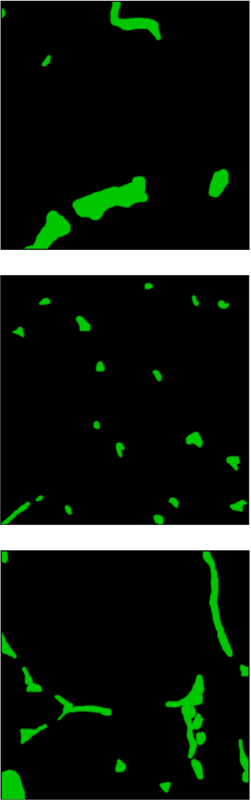
\includegraphics[width=\textwidth]{gambar/bab4/true_label.png}
		\caption{label ground truth}
		\label{fig:true_label}
	\end{subfigure}
	\hfill
	\begin{subfigure}[b]{0.24\textwidth}
		\centering
		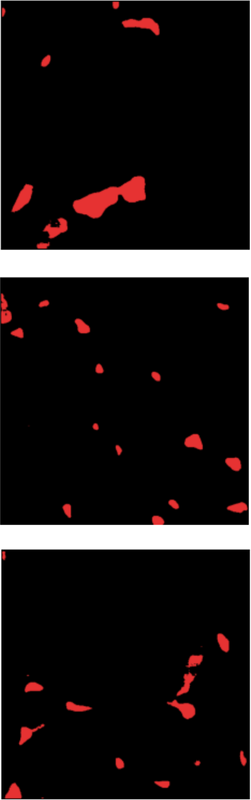
\includegraphics[width=\textwidth]{gambar/bab4/predicted_label.png}
		\caption{Prediksi model}
		\label{fig:predicted_label}
	\end{subfigure}
	\hfill
	\begin{subfigure}[b]{0.24\textwidth}
		\centering
		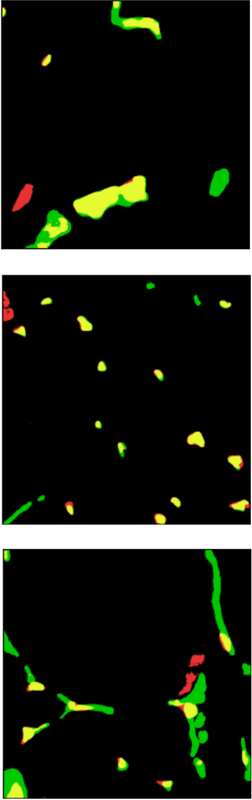
\includegraphics[width=\textwidth]{gambar/bab4/overlayed_label.png}
		\caption{Perbandingan}
		\label{fig:overlayed-label}
	\end{subfigure}
	
	\caption{Sample hasil segmentasi pada data test }
	\label{fig:sample_hasil}
	
\end{figure}

\noindent Gambar \ref{fig:sample_hasil} menunjukkan hasil segmentasi dari model Attention U-Net dibandingkan dengan ground truth. Pada panel (d), area hijau yang signifikan (false negative) terlihat pada pembuluh darah besar, menunjukkan bahwa model sering gagal mendeteksi struktur ini. Sebaliknya, area kuning (true positive) mendominasi pada pembuluh darah kecil, mencerminkan kekuatan model dalam mendeteksi struktur kecil dan terdistribusi secara lokal. Hal ini konsisten dengan nilai precision yang tinggi, tetapi recall yang lebih rendah.

\noindent Hasil evaluasi ini menunjukkan bahwa kekuatan utama model Attention U-Net terletak pada kemampuannya mendeteksi pembuluh darah kecil, yang kemungkinan disebabkan oleh mekanisme perhatian (attention mechanism) yang membantu fokus pada detail halus. Namun, tantangan terbesar model adalah mendeteksi pembuluh darah besar, yang mungkin disebabkan oleh kurangnya pembuluh darah berukuran besar berdasarkan temuan pada tahap eksplorasi data dimana data yang konsisten berukuran besar hanya ada pada dataset pertama source wsi pertama.





%\begin{table}[H]
%\centering
%\caption{Parameter kelulusan tugas akhir}
%\begin{tabular}{ clc }
%\hline
%\textbf{No.} & \textbf{Parameter } & \textbf{Nilai} \\
%\hline
%1. & Penulisan & A \\
%2. & Penulisan & A \\
%\hline
%\end{tabular}
%\label{table:nilai}
%\end{table}





% Please add the following required packages to your document preamble:
% \usepackage{booktabs}
% \usepackage{multirow}

%Berikut adalah contoh tabel yang dicetak secara horizontal
%gunakan package longtable
%Dapat dibuat dulu di https://www.tablesgenerator.com/ lalu dipindah
%\begin{landscape}
%\begin{longtable}{p{3.5cm}cllllll}
%\caption{Contoh Tabel Mendatar yang Panjang dan Lebar}\\
%\hline
%\textbf{Provinsi} & \textbf{Kode Wilayah} & \textbf{Singkatan Umum} & \textbf{ISO} & \textbf{Pulau} & \textbf{Ibu Kota} & \textbf{Gubernur} \\ \hline
%\endfirsthead

%\multicolumn{4}{l}{\bfseries \tablename\ \thetable{} -- Lanjutan dari halaman sebelumnya}\\
% \begin{center}
% % {{\bfseries \tablename\ \thetable{} -- Lanjutan dari halaman sebelumnya}} \\
% \end{center}
%\hline
%\textbf{Provinsi} & \textbf{Kode Wilayah} & \textbf{Singkatan Umum} & \textbf{ISO} & \textbf{Pulau} & \textbf{Ibu Kota} & \textbf{Gubernur} \\ \hline

%\endhead

%\hline
%\endfoot

%\endlastfoot



%Aceh & 11 & Aceh & ID-AC & Sumatera & Banda Aceh & Achmad Marzuki \\
%Sumatera Utara & 12 & Sumut & ID-SU & Sumatera & Medan & Edy Rahmayadi \\
%Sumatera Barat & 13 & Sumbar & ID-SB & Sumatera & Padang & Mahyeldi Ansharullah \\
%Riau & 14 & Riau & ID-RI & Sumatera & Pekanbaru & Syamsuar \\
%Jambi & 15 & Jambi & ID-JA & Sumatera & Jambi & Al Haris \\
%Sumatera Selatan & 16 & Sumsel & ID-SS & Sumatera & Palembang & Herman Deru \\
%Bengkulu & 17 & Bengkulu & ID-BE & Sumatera & Bengkulu & Rohidin Mersyah \\
%Lampung & 18 & Lampung & ID-LA & Sumatera & Bandar Lampung & Arinal Djunaidi \\
%Kepulauan Bangka Belitung & 19 & Babel & ID-BB & Sumatera & Pangkalpinang & Ridwan Djamaluddin \\
%Kepulauan Riau & 21 & Kepri & ID-KR & Sumatera & Tanjungpinang & Ansar Ahmad \\
%Daerah Khusus Ibukota Jakarta & 31 & DKI Jakarta & ID-JK & Jawa & Tidak ada & Heru Budi Hartono \\
%Jawa Barat & 32 & Jabar & ID-JB & Jawa & Bandung & Ridwan Kamil \\
%Jawa Tengah & 33 & Jateng & ID-JT & Jawa & Semarang & Ganjar Pranowo \\
%Daerah Istimewa Yogyakarta & 34 & DIY & ID-YO & Jawa & Yogyakarta & Hamengkubuwana X \\
%Jawa Timur & 35 & Jatim & ID-JI & Jawa & Surabaya & Khofifah Indar Parawansa \\
%Banten & 36 & Banten & ID-BT & Jawa & Serang & Al Muktabar \\
%Bali & 51 & Bali & ID-BA & Nusa Tenggara & Denpasar & I Wayan Koster \\
%Nusa Tenggara Barat & 52 & NTB & ID-NB & Nusa Tenggara & Mataram & Zulkieflimansyah \\
%Nusa Tenggara Timur & 53 & NTT & ID-NT & Nusa Tenggara & Kupang & Viktor Laiskodat \\

%Kalimantan Barat & 61 & Kalbar & ID-KB & Kalimantan & Pontianak & Sutarmidji \\
%Kalimantan Tengah & 62 & Kalteng & ID-KT & Kalimantan & Palangka Raya & Sugianto Sabran \\
%Kalimantan Selatan & 63 & Kalsel & ID-KS & Kalimantan & Banjarbaru & Sahbirin Noor \\
%Kalimantan Timur & 64 & Kaltim & ID-KI & Kalimantan & Samarinda & Isran Noor \\
%Kalimantan Utara & 65 & Kaltara & ID-KU & Kalimantan & Tanjung Selor & Zainal Arifin Paliwang \\
%Sulawesi Utara & 71 & Sulut & ID-SA & Sulawesi & Manado & Olly Dondokambey \\
%Sulawesi Tengah & 72 & Sulteng & ID-ST & Sulawesi & Palu & Rusdy Mastura \\
%Sulawesi Selatan & 73 & Sulsel & ID-SN & Sulawesi & Makassar & Andi Sudirman Sulaiman \\
%Sulawesi Tenggara & 74 & Sultra & ID-SG & Sulawesi & Kendari & Ali Mazi \\
%Gorontalo & 75 & Gorontalo & ID-GO & Sulawesi & Gorontalo & Hamka Hendra Noer \\
%Sulawesi Barat & 76 & Sulbar & ID-SR & Sulawesi & Mamuju & Akmal Malik \\
%Maluku & 81 & Maluku & ID-MA & Maluku & Ambon & Murad Ismail \\
%Maluku Utara & 82 & Malut & ID-MU & Maluku & Sofifi & Abdul Ghani Kasuba \\
%Papua & 91 & Papua & ID-PA & Papua & Jayapura & Lukas Enembe \\
%Papua Barat & 92 & Pabar & ID-PB & Papua & Manokwari & Paulus Waterpauw \\
%Papua Selatan & 93 & Pasel & — & Papua & Merauke & Apolo Safanpo \\
%Papua Tengah & 94 & Papteng & — & Papua & Nabire & Ribka Haluk \\
%Papua Pegunungan & 95 & Papeg & — & Papua & Wamena & Nikolaus Kondomo \\
%Papua Barat Daya & 96 & PBD & — & Papua & Sorong1 & — \\ \hline
%\label{table:tabelpanjanglebar}
%\end{longtable}
%\end{landscape}


%		\subsection{Subsubbab 2 2}
%		\blindtext

%	\section{Subab 3}
%	\blindtext \ref{fig:komputer}

%\begin{equation}
 %   x+2 = 159
%\end{equation}
%\blindtext

%Berikut adalah contoh gambar yang dicetak secara horizontal
%\begin{landscape}
 %  \begin{figure}[t]
  %      \centering
   %     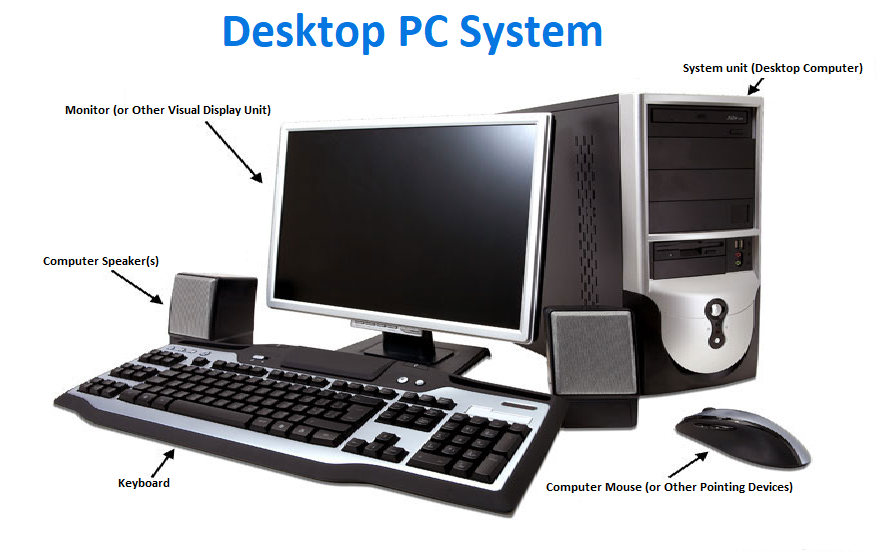
\includegraphics[width=18cm, height=12cm]{gambar/contoh-gambar-miring.png}
    %    \caption{Contoh Gambar Komputer}
     %   \label{fig:komputer}
    %\end{figure}
%\end{landscape}

